%%%%%%%%%%%%%%%%%%%%%%%%%%%%%%%%%%%%%%%%%
% Lachaise Assignment
% LaTeX Template
% Version 1.0 (26/6/2018)
%
% This template originates from:
% http://www.LaTeXTemplates.com
%
% Authors:
% Marion Lachaise & François Févotte
% Vel (vel@LaTeXTemplates.com)
%
% License:
% CC BY-NC-SA 3.0 (http://creativecommons.org/licenses/by-nc-sa/3.0/)
% 
%%%%%%%%%%%%%%%%%%%%%%%%%%%%%%%%%%%%%%%%%



%----------------------------------------------------------------------------------------
%	PACKAGES AND OTHER DOCUMENT CONFIGURATIONS
%----------------------------------------------------------------------------------------

\documentclass{article}

\usepackage{dirtree}

\usepackage{hyperref}

\usepackage{listings}

%%%%%%%%%%%%%%%%%%%%%%%%%%%%%%%%%%%%%%%%%
% Lachaise Assignment
% Structure Specification File
% Version 1.0 (26/6/2018)
%
% This template originates from:
% http://www.LaTeXTemplates.com
%
% Authors:
% Marion Lachaise & François Févotte
% Vel (vel@LaTeXTemplates.com)
%
% License:
% CC BY-NC-SA 3.0 (http://creativecommons.org/licenses/by-nc-sa/3.0/)
% 
%%%%%%%%%%%%%%%%%%%%%%%%%%%%%%%%%%%%%%%%%

%----------------------------------------------------------------------------------------
%	PACKAGES AND OTHER DOCUMENT CONFIGURATIONS
%----------------------------------------------------------------------------------------

\usepackage{amsmath,amsfonts,stmaryrd,amssymb} % Math packages

\usepackage{enumerate} % Custom item numbers for enumerations

\usepackage[ruled]{algorithm2e} % Algorithms

\usepackage[framemethod=tikz]{mdframed} % Allows defining custom boxed/framed environments

\usepackage{listings} % File listings, with syntax highlighting
\lstset{
	basicstyle=\ttfamily, % Typeset listings in monospace font
}

%----------------------------------------------------------------------------------------
%	DOCUMENT MARGINS
%----------------------------------------------------------------------------------------

\usepackage{geometry} % Required for adjusting page dimensions and margins

\geometry{
	paper=a4paper, % Paper size, change to letterpaper for US letter size
	top=2.5cm, % Top margin
	bottom=3cm, % Bottom margin
	left=2.5cm, % Left margin
	right=2.5cm, % Right margin
	headheight=14pt, % Header height
	footskip=1.5cm, % Space from the bottom margin to the baseline of the footer
	headsep=1.2cm, % Space from the top margin to the baseline of the header
	%showframe, % Uncomment to show how the type block is set on the page
}

%----------------------------------------------------------------------------------------
%	FONTS
%----------------------------------------------------------------------------------------

\usepackage[utf8]{inputenc} % Required for inputting international characters
\usepackage[T1]{fontenc} % Output font encoding for international characters

\usepackage{XCharter} % Use the XCharter fonts

%----------------------------------------------------------------------------------------
%	COMMAND LINE ENVIRONMENT
%----------------------------------------------------------------------------------------

% Usage:
% \begin{commandline}
%	\begin{verbatim}
%		$ ls
%		
%		Applications	Desktop	...
%	\end{verbatim}
% \end{commandline}

\mdfdefinestyle{commandline}{
	leftmargin=10pt,
	rightmargin=10pt,
	innerleftmargin=15pt,
	middlelinecolor=black!50!white,
	middlelinewidth=2pt,
	frametitlerule=false,
	backgroundcolor=black!5!white,
	frametitle={Command Line},
	frametitlefont={\normalfont\sffamily\color{white}\hspace{-1em}},
	frametitlebackgroundcolor=black!50!white,
	nobreak,
}

% Define a custom environment for command-line snapshots
\newenvironment{commandline}{
	\medskip
	\begin{mdframed}[style=commandline]
}{
	\end{mdframed}
	\medskip
}

%----------------------------------------------------------------------------------------
%	FILE CONTENTS ENVIRONMENT
%----------------------------------------------------------------------------------------

% Usage:
% \begin{file}[optional filename, defaults to "File"]
%	File contents, for example, with a listings environment
% \end{file}

\mdfdefinestyle{file}{
	innertopmargin=1.6\baselineskip,
	innerbottommargin=0.8\baselineskip,
	topline=false, bottomline=false,
	leftline=false, rightline=false,
	leftmargin=2cm,
	rightmargin=2cm,
	singleextra={%
		\draw[fill=black!10!white](P)++(0,-1.2em)rectangle(P-|O);
		\node[anchor=north west]
		at(P-|O){\ttfamily\mdfilename};
		%
		\def\l{3em}
		\draw(O-|P)++(-\l,0)--++(\l,\l)--(P)--(P-|O)--(O)--cycle;
		\draw(O-|P)++(-\l,0)--++(0,\l)--++(\l,0);
	},
	nobreak,
}

% Define a custom environment for file contents
\newenvironment{file}[1][File]{ % Set the default filename to "File"
	\medskip
	\newcommand{\mdfilename}{#1}
	\begin{mdframed}[style=file]
}{
	\end{mdframed}
	\medskip
}

%----------------------------------------------------------------------------------------
%	NUMBERED QUESTIONS ENVIRONMENT
%----------------------------------------------------------------------------------------

% Usage:
% \begin{question}[optional title]
%	Question contents
% \end{question}

\mdfdefinestyle{question}{
	innertopmargin=1.2\baselineskip,
	innerbottommargin=0.8\baselineskip,
	roundcorner=5pt,
	nobreak,
	singleextra={%
		\draw(P-|O)node[xshift=1em,anchor=west,fill=white,draw,rounded corners=5pt]{%
		Question \theQuestion\questionTitle};
	},
}

\newcounter{Question} % Stores the current question number that gets iterated with each new question

% Define a custom environment for numbered questions
\newenvironment{question}[1][\unskip]{
	\bigskip
	\stepcounter{Question}
	\newcommand{\questionTitle}{~#1}
	\begin{mdframed}[style=question]
}{
	\end{mdframed}
	\medskip
}

%----------------------------------------------------------------------------------------
%	WARNING TEXT ENVIRONMENT
%----------------------------------------------------------------------------------------

% Usage:
% \begin{warn}[optional title, defaults to "Warning:"]
%	Contents
% \end{warn}

\mdfdefinestyle{warning}{
	topline=false, bottomline=false,
	leftline=false, rightline=false,
	nobreak,
	singleextra={%
		\draw(P-|O)++(-0.5em,0)node(tmp1){};
		\draw(P-|O)++(0.5em,0)node(tmp2){};
		\fill[black,rotate around={45:(P-|O)}](tmp1)rectangle(tmp2);
		\node at(P-|O){\color{white}\scriptsize\bf !};
		\draw[very thick](P-|O)++(0,-1em)--(O);%--(O-|P);
	}
}

% Define a custom environment for warning text
\newenvironment{warn}[1][Warning:]{ % Set the default warning to "Warning:"
	\medskip
	\begin{mdframed}[style=warning]
		\noindent{\textbf{#1}}
}{
	\end{mdframed}
}

%----------------------------------------------------------------------------------------
%	INFORMATION ENVIRONMENT
%----------------------------------------------------------------------------------------

% Usage:
% \begin{info}[optional title, defaults to "Info:"]
% 	contents
% 	\end{info}

\mdfdefinestyle{info}{%
	topline=false, bottomline=false,
	leftline=false, rightline=false,
	nobreak,
	singleextra={%
		\fill[black](P-|O)circle[radius=0.4em];
		\node at(P-|O){\color{white}\scriptsize\bf i};
		\draw[very thick](P-|O)++(0,-0.8em)--(O);%--(O-|P);
	}
}

% Define a custom environment for information
\newenvironment{info}[1][Info:]{ % Set the default title to "Info:"
	\medskip
	\begin{mdframed}[style=info]
		\noindent{\textbf{#1}}
}{
	\end{mdframed}
}
 % Include the file specifying the document structure and custom commands


%----------------------------------------------------------------------------------------
%	ASSIGNMENT INFORMATION
%----------------------------------------------------------------------------------------

\title{Spark on Amazon Web Services} % Title of the assignment

%\author{David Domingo\\ \texttt{djd240@cs.rutgers.edu}} % Author name and email address

\date{\vspace{-8ex}} % University, school and/or department name(s) and a date


%----------------------------------------------------------------------------------------

\begin{document}

\maketitle % Print the title


\begin{figure}[h!]
 \centering
 
\includegraphics[width=50mm]{images/Apache_Spark_logo.png}\hspace{15mm}
 
\includegraphics[width=60mm]{images/AWS}
\end{figure} 

%----------------------------------------------------------------------------------------
%	INTRODUCTION
%----------------------------------------------------------------------------------------

\section*{Introduction} % Unnumbered section

In this guide, we'll be going over how to use Amazon Web Service's Elastic MapReduce to run MapReduce jobs. Elastic MapReduce (a.k.a EMR) is Amazon's solution to data analytics based on Hadoop. Users can create clusters running Hadoop and run distributed MapReduce/Spark programs. This guide covers how to set up your own Hadoop cluster using AWS EMR, how to interact with the Hadoop Cluster, and how to run MapReduce Jobs.

%----------------------------------------------------------------------------------------
%	TABLE OF CONTENTS
%----------------------------------------------------------------------------------------

\hypersetup{hidelinks}
\tableofcontents

%----------------------------------------------------------------------------------------
%	Setting up AWS
%----------------------------------------------------------------------------------------

\section{Setting up AWS}
\subsection{Signing up for AWS}
In order to use EMR, you need an AWS account to access AWS's services. If don't have an AWS account already,  you can sign up at https://portal.aws.amazon.com/billing/signup . Note: You will need to a credit card to sign up for an AWS account. 
\subsection{Getting Educational Credit}
Now that you have an AWS account, you need credit so you can use AWS services without being charged on out credit cards. Currently, Amazon will give \$100 of free credit which should be more than enough to run a Hadoop Cluster for 100+ hours. To do this, 
\begin{enumerate}
    \item Go to https://aws.amazon.com/education/awseducate/
    \item Click "Join AWS Educate" to start registering
    \item Fill out the form accordingly. Ensure you use your school .edu email and leave the promo code field empty
    \item You will notice there are two options. Select the first one to use the AWS account you created.
    \item Enter your AWS Account ID. You can find this by logging into AWS, selecting your name at the top of the page, and clicking "My Account". Under the account setting section on your account page, your account id should be listed. 
    \item Click "Next"
    \item Read the Terms and Conditions, select "I Agree", and click submit. 
    \item After AWS reviews your application, you should get an email with a credit code worth \$100 dollars.
    \item To add the credit to your account, follow the directions in the email.
\end{enumerate}

\begin{info}[Sign up time:]
AWS has review your educational credit application before you receive any credit. This could take from a few minutes to a few hours. 
\end{info}

\begin{info}[Free educational account with no credit card:]
It is possible to sign up for a free AWS educate account but it is limited and you can not keep running anything when the limits have been reached. It is recommended to sign up with a regular AWS account and apply for educational credit so you are not bound by any limits. The \$100 of AWS credit you receive should be more than enough to last you the duration of your project around 100 hours of cluster uptime).
\end{info}

%----------------------------------------------------------------------------------------
%	CLUSTER MANAGEMENT
%----------------------------------------------------------------------------------------

\section{Cluster Management}

\subsection{Creating a Security Key-Pair}
When you create your own Hadoop cluster, it will open to the internet and you will able to access it from anywhere. You should create a security key pair so when you do create any clusters, you can configure it to only accept incoming connections from those who have the key. To create a key-pair, do the following:

\begin{enumerate}
    \item Go to https://us-west-2.console.aws.amazon.com/ec2/home
    \item On the left hand panel, under "NETWORK \& SECURITY", click "Key Pairs"
    \item Start creating a key pair by clicking "Create Key Pair"
    \item Name it the new key pair and click "Create".
    \item The key pair will be created and your browser should prompt you to download the key (.pem file). Save this in a safe space, you will need this for when you SSH or SCP to the cluster. 
\end{enumerate}

\begin{info}[Using AWS without keys:]
It is possible to configure clusters to not need a key to access. This is not recommended.
\end{info}


\subsection{Starting your cluster}
In order to start a new cluster, do the following:
\begin{enumerate}
    \item Go to AWS EMR by going to Services,  and under the "Analytics" section, click "EMR".
    \item On the EMR home page, click "Create Cluster".
    \item Within the cluster configuration page, give your cluster a name.
    \item Under the Software Configuration Section, make sure Core Hadoop is selected under Applications
    \item Under the Hardware Configuration Section, make sure "m3.xlarge" in the dropdown. This is the default size. This should be enough for typical usage.
    \item Under Security and access, if you made a security key-pair, select the key-pair you made in the EC2 key pair dropdown.
    \item Click "Create cluster".
    \item Now to connect to remotely your cluster follow the next section to add security rules for you cluster. 
\end{enumerate}
\begin{info}[Startup Time:]
When starting a cluster, it typically takes some time for the hardware resources to be allocated and functionalities set up for your cluster. It could possibly take to up to 15-20 minutes for your cluster to start.
\end{info}
\subsection{Setting Security Rules}
\noindent By default, you won't be able to connect to your cluster. In order to connect to the cluster you have to manually add security rules in order for you to connect via SSH, TCP, and ICMP protocols over the internet. To do this, do the following:
\begin{enumerate}
     \item On the Amazon EMR dashboard, navigate to your cluster by clicking its name.
     \item Within the summary tab for your cluster, under the "Security and Access" section, click the link following "Security groups for Master"
     \item Select the entry for ElasticMapReduce-master.
     \item Navigate to the "Inbound" tab below and click "Edit"
     \item Add a rule for TCP by clicking "Add Rule", selecting "All TCP" in the type dropdown, and selecting "Anywhere" in the source dropdown.
     \item Add a rule for ICMP by clicking "Add Rule", selecting "All ICMP - IPv4" in the type dropdown, and selecting "Anywhere" in the source dropdown.
     \item Finally, add a final rule for SSH by clicking "Add Rule", selecting "SSH" in the type dropdown, and selecting "Anywhere" in the source dropdown.
     \item Save the rules you just created by clicking "Save".
\end{enumerate}
\subsection{Terminating a Cluster}
To terminate/shut down a cluster you started, do the following:
\begin{enumerate}
    \item Go the EMR Home and go to Clusters
    \item Select the cluster you want to terminate and click "Terminate"
\end{enumerate}
\begin{info}[You will lose everything:]
Note that when you terminate your cluster, you will lose everything you have stored on the cluster. Make sure to copy anything that you need back to your machine or use Amazon S3 buckets to persist data between cluster sessions. (We'll go over S3 bucket a little later in this document)
\end{info}
\begin{info}[Shut Down Time:]
It could possibly take a few minutes to shut down a cluster.
\end{info}
\subsection{Restarting a Cluster}
Since AWS allocates resources for your cluster on demand, there no such thing as "restarting" a cluster. Once it's gone, it's gone. What you can do is clone a previous cluster to start a new cluster with the same cluster configuration. To do this, 
\begin{enumerate}
    \item Go to the EMR home and go to clusters. 
    \item Select the cluster you want to clone
    \item Click "Clone"
\end{enumerate}
\subsection{Tips for Cluster Usage}
\subsubsection{Avoiding Unnecessary Charges}
To avoid unnecessary charges, make sure you terminate your cluster whenever you are not going to use your cluster. It would be fine to leave the cluster running if you wont be using the cluster for 30 minutes or so. 
\subsubsection{Checking Cluster Usage}
You can check your billing forecast on AWS by clicking your name at the top and clicking "My billing dashboard". It should bring you to your billing dashboard, showing the expected cost based on your current cluster usage.
\subsubsection{Sharing the Cluster}
It may be more efficient for you to share a single cluster if you are perhaps working a group. In order to do this you can just share the secret key with anyone else that you want to share the cluster with. You could also start the cluster with no security. But this is highly not recommended.
\subsubsection{Cleaning up after use}
When you are done using AWS EMR, make sure to terminate any running clusters and delete any S3 data you may have stored. This will ensure you won't be charged for any AWS usage in the future.


%----------------------------------------------------------------------------------------
%	RUNNING MAPREDUCE
%----------------------------------------------------------------------------------------

\section{Running MapReduce}
In order to run MapReduce you will have do three things. Place your jar somewhere the cluster can access it. Place the input data somewhere the cluster could access. Run MapReduce. 
\subsection{Connecting to the Cluster}
You run commands on the EMR cluster, you can connect the the EMR cluster with SSH. To connect to your cluster you will use connect as Hadoop at master public DNS. You can find the master public DNS of your cluster under the summary section for your cluster.
\begin{lstlisting}[language=bash]
  $ ssh -i <key location> <remote>
\end{lstlisting}
example:
\begin{lstlisting}[language=bash]
  $ ssh -i mykey.pem hadoop@ec2-54-245-34-159.us-west-2.compute.amazonaws.com
\end{lstlisting}

\begin{info}[Make sure you added security rules:]
If you can not connect to your cluster, ensure that you have added the proper security rules to allow you to connect. You can find out how to do this in section 2.3. 
\end{info}

\subsection{Ways to run MapReduce }
In order to run MapReduce, you have to have files accessible to the cluster. You have two options when it comes to running MapReduce: 
\begin{enumerate} 
\item Store your files directly onto the cluster using scp and use hdfs commands to move files to hdfs. You will have to run thee Hadoop program by executing a command on the cluster via SSH. 
\item Upload your files in Amazon S3 buckets and have Hadoop pull the data from there. You will to run a MapReduce Job by using Amazon EMR Steps.
\end{enumerate}

\subsection{Running MapReduce Manually using SSH, SCP, and Hadoop Commands}
The following section the traditional way of running MapReduce, covering how you would typically interact with a Hadoop Cluster.

\subsubsection{Manually Storing Files on Hadoop Cluster}
In order to run MapReduce you'll need to put your runnable jar and input files onto the cluster. You can transfer files to your cluster by using the scp command. Typical usage is as follows:
\begin{lstlisting}[language=bash]
  $ scp <source> <destination>
\end{lstlisting} 
Since you need a key to connect to your cluster you will need to pass the key to the command using the -i flag:
\begin{lstlisting}[language=bash]
  $ scp -i <key location> <source> <destination>
\end{lstlisting}
Example:
\begin{lstlisting}[language=bash]
  $ scp -i mykey.pem WordCount.jar 
    hadoop@ec2-54-245-34-159.us-west-2.compute.amazonaws.com:~
\end{lstlisting}
\-\\\ \textbf{Note:} Notice the usage of the colon within the destination. The path after the colon specifies the file path the file should be placed on the destination system. In our example we simply used the tilde character, $\sim$, which represents the home directory.

\-\ \\ You can see more about how to use scp here: https://haydenjames.io/linux-securely-copy-files-using-scp/

\subsubsection{Getting Files Input Files into HDFS}
Now for Hadoop to use your input, the input files must be on HDFS. By using scp you were able to get your files onto the machine, but not onto HDFS. Now you need to get it from the machine to HDFS. To get it on HDFS, use HDFS commands to move files to and from HDFS while SSH'd in the cluster.

\-\\\ You can move a file to hdfs by using the -put command:
\begin{lstlisting}[language=bash]
  $ hdfs dfs -put <source> <dest>
\end{lstlisting}    
You can list your files on hdfs by using the -ls command:
\begin{lstlisting}[language=bash]
  $ hdfs dfs -ls 
\end{lstlisting} 
Example:
\begin{lstlisting}[language=bash]
  $ ls
  input.txt
  $ hdfs dfs -put input.txt 
  $ hdfs dfs -ls 
  Found 1 item 
  -rw-r--r--   1 hadoop hadoop          0 2018-11-20 00:17 input.txt
\end{lstlisting} 

\-\ \\ You can read more on HDFS commands here:\\ https://hadoop.apache.org/docs/r2.4.1/hadoop-project-dist/hadoop-common/FileSystemShell.html
 
 \subsubsection{Manually Running MapReduce Using Hadoop Jar}
To run the MapReduce program, while SSH'd into the cluster, invoke Hadoop to run MapReduce by using the Hadoop jar command:
\begin{lstlisting}[language=bash]
  $ hadoop jar <jar location> <Main Class> <input> <output>
\end{lstlisting}
Example with the runnable jar on the cluster, the input data named input.txt in HDFS, and specifying Hadoop to create a folder named "output" to put the output files in:
\begin{lstlisting}[language=bash]
  $ hadoop jar WordCount-0.0.1-SNAPSHOT.jar WordCount input.txt output
\end{lstlisting}


\begin{info}[Output must be Unique:]
When specifying the output folder, make sure the folder name is unique and unused. If there already exists a folder with the same name, MapReduce will not run successfully as Hadoop won't be able to create a folder with a name that already exists.
\end{info}

 \begin{info}[You will lose everything:]
Remember every time you terminate your cluster, everything stored on the cluster will be gone. Make sure to copy back any files you will need.
\end{info}

 
\subsection{Running MapReduce using S3 Buckets and EMR steps}
In order to make it easier for users, Amazon provides seamless integration with AWS S3 and the your EMR Hadoop Cluster as a means to run MapReduce without having to SSH into the cluster and run commands to move files around.
\subsubsection{Storing files in S3 Buckets}
Instead of storing putting data on the cluster you can instead upload our data to an AWS S3 bucket. AWS S3 is AWS's storage solution. You may find it easier and more helpful to store data in the S3 buckets in order to persist any of our data. To do this
\begin{enumerate} 
    \item Go to "Services" at the top of the page and under the "Storage" section, click "S3". 
    \item Create a new bucket to store files in. 
    \item Use the web interface to upload your files.
\end{enumerate}


\subsubsection{Adding A Step to the Cluster}
You can invoke MapReduce without having to SSH into the cluster by utilizing AWS EMR's step interface. To do this do the following:
\begin{enumerate}
    \item Go to the EMR home.
    \item Go to clusters in the sidebar. 
    \item Click the cluster you are running. 
    \item Go to the steps tab.
    \item Click "Add Step"
    \item Select "Custom JAR" within the Step type dropdown.
    \item For the location box, navigate to the jar file you stores on S3, or if you stored it on HDFS manually, enter the file location on HDFS.
    \item Enter the jar arguments like you would if you did it manually, specifying the java Class to run, the input, and output.
\end{enumerate}
Example:
\begin{figure}[h!]
 \centering
 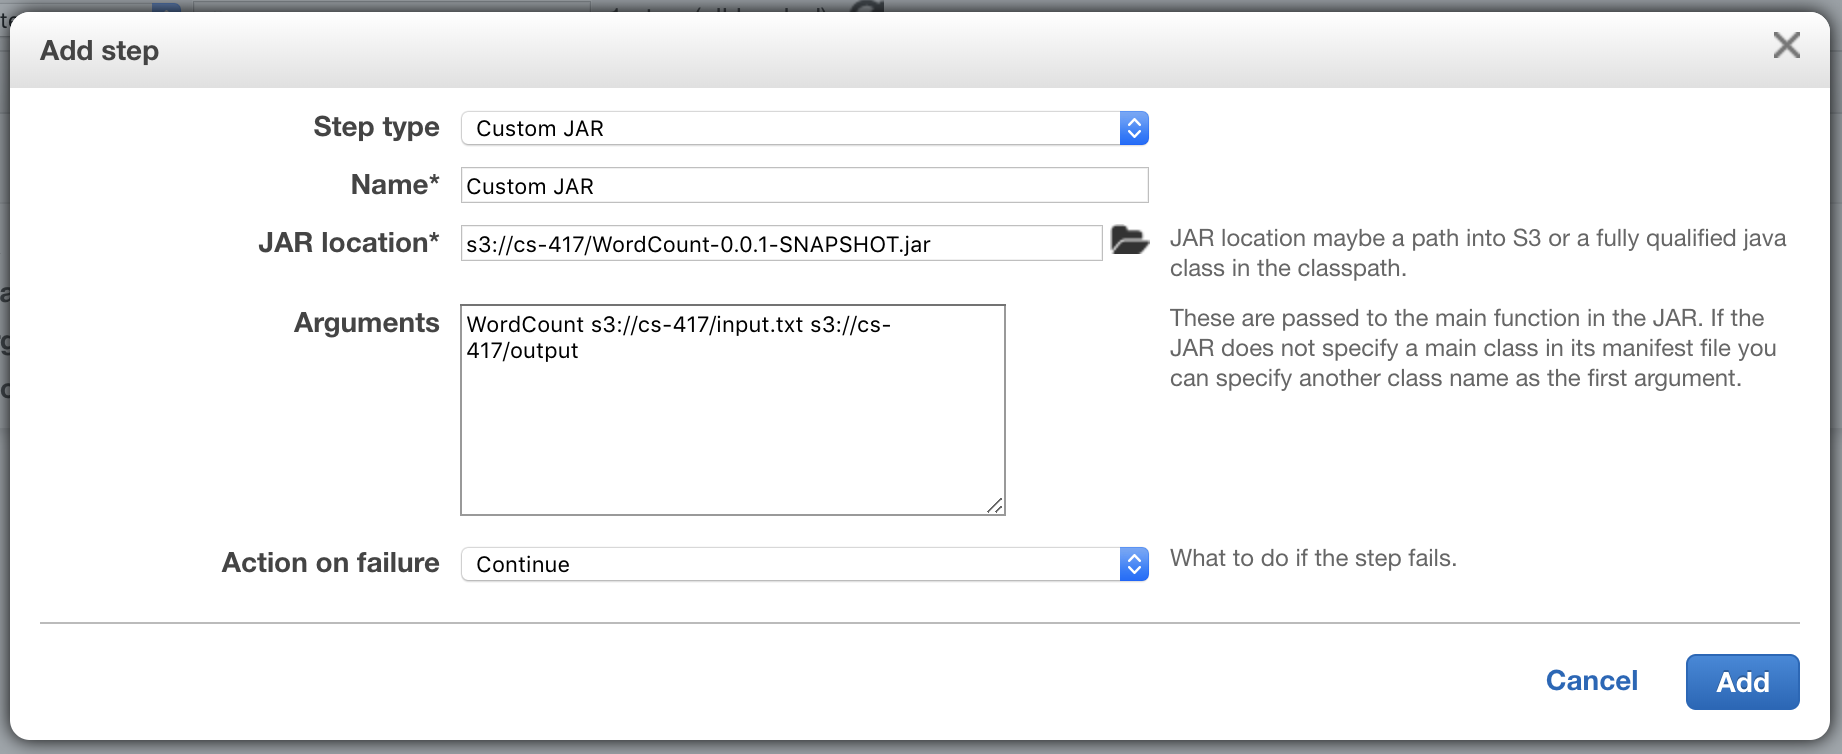
\includegraphics[width=150mm]{images/step}
\end{figure} 
\-\ \\\textbf{Note:} Notice how files within your S3 bucket are referenced. In this case we're invoking the Word Count Runnable jar passing in arguments, giving it the location of our input file "input.txt" located within our "cs-417" S3 bucket. We then specify Hadoop to place the results in a folder called "output" in our S3 bucket.

\begin{info}[Output must be Unique:]
Even on Amazon S3, when specifying the output folder, make the output folder name unique. If there already exists a folder with the same name, MapReduce will not run successfully as Hadoop won't be able to create a folder with a name that already exists.
\end{info}


\subsection{Analyzing MapReduce Output}
To view the results of the MapReduce program, check out the resulting files Hadoop created in the output folder you specified.
\subsubsection{Checking out Results in Secure Shell}
If you ran the MapReduce manually, invoking Hadoop within an SSH session. You can checkout the output by using the hdfs ls and cat commands.
For example if you specified Hadoop to store the results in a folder called "output" on HDFS, you can list the files within the output folder using the ls command
\begin{lstlisting}[language=bash]
  $ hdfs dfs -ls output
  -rw-r--r--   1 hadoop hadoop          0 2018-11-20 00:06 output4/_SUCCESS
  -rw-r--r--   1 hadoop hadoop      49831 2018-11-20 00:06 output/part-r-00000
  -rw-r--r--   1 hadoop hadoop      49924 2018-11-20 00:06 output/part-r-00001
\end{lstlisting}
You can then print out the contents of one of the result files by using the cat command
\begin{lstlisting}[language=bash]
  $ hdfs dfs -cat output/part-r-00000
\end{lstlisting}
If you want to copy the results from HDFS back to your cluster, you can use the hdfs get command:
 \begin{lstlisting}[language=bash]
  $ hdfs dfs -get output/part-r-00000
\end{lstlisting} 
If you want to transfer the results back to your local computer (not the cluster machine), you can use a combination of the scp command like when you transferred files to the cluster, but instead switching the source and destination locations.

\subsubsection{Checking out Results Stored on S3}
If you specified Hadoop to store the results in your S3 bucket, you can checkout the results by navigating to your S3 buckets and downloading the resulting files.


%----------------------------------------------------------------------------------------
%	USEFUL LINKS AND RESOURCES
%----------------------------------------------------------------------------------------
\section{Useful links and Resources}
\textbf{Hadoop Cluster Interaction}
\begin{itemize}
    \item \textit{HDFS Overview and Commands}\\ https://hadoop.apache.org/docs/r2.4.1/hadoop-project-dist/hadoop-common/FileSystemShell.html
\end{itemize}
\textbf{MapReduce Guides}
\begin{itemize}
    \item \textit{Apache MapReduce Tutorial}\\ https://hadoop.apache.org/docs/stable/hadoop-mapreduce-client/hadoop-mapreduce-client-core/\\MapReduceTutorial.html
\end{itemize} 



\-\\\\\\\\\\\\\noindent \date{Last Updated: \today}

%\begin{info}[Testing your web service:]
%There are multiple tools you can use to make HTTP requests. Use these tools to test your web service
%\end{info}

%% File contents
%\begin{file}[hello.py]
%\begin{lstlisting}[language=Python]
%#! /usr/bin/python
%
%import sys
%sys.stdout.write("Hello World!\n")
%\end{lstlisting}
%\end{file}

\end{document}
